\documentclass{deck}
\usepackage[american]{babel}
\usepackage{merriweather}
\begin{document}

\slide{
  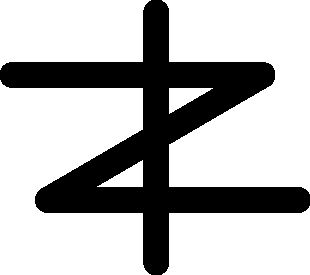
\includegraphics[scale=1]{../images/zerocracy-logo.pdf}\\
  Zerocracy, Inc.
  \\[1em]
  \large
  Freelance vs. Outsourcing\\
  \href{https://www.zerocracy.com}{www.zerocracy.com}
}

\newcommand\topic[3]{\vbox{\raggedright{\normalsize\colorbox{#1}{\color{white}{#2}}}\newline\footnotesize#3\vspace{4pt}}}

\slide{
  \newcommand{\dt}[2]{
    \draw +(0,#1)
      node[circle, inner sep=0mm, minimum width=3pt, fill=zblue, draw=none] {}
      node[anchor=east] {\scriptsize #1}
      node[anchor=west] {\scriptsize #2};
  }
  \newcommand\graph[1]{\vbox{
    \begin{tikzpicture}[y=0.16cm]
      \draw[-triangle 60] +(0,1968) -- +(0,2018);
      #1
    \end{tikzpicture}
  }}
  The Evolution of Software Development:
  \begin{multicols}{2}
    \graph{
      \dt{1970}{Waterfall}
      \dt{1980}{V-Model}
      \dt{1982}{CASE}
      \dt{1987}{PMBOK}
      \dt{1989}{PRINCE2}
      \dt{1991}{RAD}
      \dt{1993}{MSF}
      \dt{1995}{Scrum}
      \dt{1999}{XP}
      \dt{2001}{Agile}
      \dt{2003}{RUP}
      \dt{2010}{\colorbox{zgreen}{\color{white}{XDSD}}}
    }
    \graph{
      \dt{1970}{Capgemini}
      \dt{1975}{Wipro}
      \dt{1989}{Accenture}
      \dt{1993}{EPAM Systems}
      \dt{1999}{Elance/oDesk/Upwork}
      \dt{2001}{Crossover}
      \dt{2010}{Toptal}
      \dt{2016}{\colorbox{zgreen}{\color{white}{Zerocracy}}}
    }
  \end{multicols}
  \Large
  eXtremely Distributed Software Development (\href{https://www.xdsd.org}{XDSD}) methodology was
  invented by Yegor Bugayenko in 2010. Six years later he founded
  Zerocracy in order to apply XDSD to the growing market of freelancers.
}

\slide{
  Gallup \href{https://www.cnbc.com/2018/05/30/70-percent-of-people-globally-work-remotely-at-least-once-a-week-iwg-study.html}{recently found out}
  that the number of American employees
  working remotely rose to 43 percent in 2016 from 39 percent in 2012.
  However, as \href{https://www.entrepreneur.com/article/280749}{noted}
  by Rustam Singh in Entrepreneur,
  ``freelancers are exactly second in line (right after interns),
  to be regarded as the most \underline{under-appreciated} working population
  on the planet currently.''
}

\slide{
  What Are the Key Freelance Pitfalls?
  \begin{multicols}{3}
  \topic{zred}{Lack of Control}{
    Qubit Labs, a Ukrainian outsourcer, in their blog post of disappointed
    \href{https://qubit-labs.com/reasons-why-we-will-never-hire-freelancers-again/}{explains}:
    ``You do not know exactly how freelancer works. No matter how
    much you convince yourself, you have no power over freelancers.
    They can deliver the project on time, or not.''}

  \topic{zred}{Low Quality}{
    It is often assumed that programmers working remotely without
    close daily supervision produce lower quality of their code
    than their full-time colleagues.}

  \topic{zred}{Communication Issues}{
    Reddit and Yahoo \href{http://www.gallup.com/poll/184649/telecommuting-work-climbs.aspx}{banned}
    remote work and Reddit CEO
    \href{https://www.quora.com/Is-Reddit-closing-their-NYC-and-Salt-Lake-City-offices-They-have-asked-all-remote-workers-to-decide-by-the-end-of-2014-if-they-want-to-move-to-San-Francisco-or-leave-the-company}{said}
    that
    ``there were too many times when we just needed to be able
    to walk over and tap someone on the shoulder and discuss
    a complex issue in-depth, right away,'' which is difficult
    to do with remotely distributed freelancers.}

  \topic{zred}{Fake Portfolios}{
    Relja Damnjanovic from \href{https://www.toptal.com}{Toptal} describes his personal experience of
    being a victim of identity theft and
    \href{https://www.toptal.com/freelance/freelancer-identity-theft}{says} that,
    ``Unethical people create profiles on open freelance networks,
    pretending to be someone with much more experience and expertise
    than themselves. They use the stolen profile to poach
    jobs, and set higher prices than they're worth.''}

  \topic{zred}{IPR Issues}{
    While full-time employees are binded by multi-page NDAs and contracts,
    freelancers, even when they ``work for hire'' are less responsible legally;
    moreover, they are mostly overseas.}

  \topic{zred}{High Turnover}{
    As Riia O'Donnell from RecruiterBox
    \href{https://recruiterbox.com/blog/freelance-vs-fulltime-pros-cons-hiring-independent-contractor}{says},
    ``They may be great when they're accessible,
    but be prepared with a Plan B if they're not.''}

  \topic{zred}{Absence of Talents}{
    As \href{https://en.wikipedia.org/wiki/Yishan_Wong}{Yishan Wong},
    former CEO of Reddit, \href{https://www.quora.com/How-does-a-business-person-outsource-a-good-developer-programmer-engineer-on-eLance-or-oDesk-I-dont-understand-nor-can-I-differentiate-all-the-latest-programming-languages-What-skill-sets-should-I-be-looking-for/answer/Yishan-Wong}{described}
    his freelance experience, ``it was extremely difficult to find decent engineers who could
    do the things he needed, deliver reliably, and iterate according
    to ongoing testing/customer feedback.''}

  \topic{zred}{Lack of Commitment}{
    ``If client site is down, a client can't call a freelancer
    to work on it right at this moment but it's different for an employee,''
    \href{https://imtips.co/disadvantages-hiring-freelancer.html}{says} Shabbir Bhimani,
    a software blogger.}

  \topic{zred}{No Accountability}{
    ``A lot of freelancers have no drive and determination, it is
    self-motivated job and if they are having a bad day then it
    is so easy to see why they may not produce high standard work,''
    \href{https://creativebeacon.com/freelancers-bad-reputation/}{says} Creative Beacon.}

  \topic{zred}{Good Ones Are Expensive}{
    Even though the \href{https://vulcanpost.com/634361/freelancer-singapore-paypal-survey/}{recent study}
    of PayPal revealed that over 50\% of freelancers are not being paid regularly,
    in order to hire a decent engineer one has to pay double, since,
    as Jay Soriano \href{http://launchastartup.com/odesk-vs-elance/}{explained},
    ``the good freelancers become insulted with the low pricing, and
    the `good enough' freelancers stay but don't feel that they
    have to provide quality because the price is so low.''}

  \topic{zred}{Cultural Differences}{
    Anne Loehr claims in her
    \href{https://www.anneloehr.com/2014/11/03/4-steps-maintain-organizational-culture-freelance-employees/}{blog post} that
    ``freelance employees don't fit in with the organizational culture'' and it's a ``management challenge.''}

  \topic{zred}{Moody Attitude}{
    As Sara Horowitz, founder of \href{https://www.freelancersunion.org/}{Freelancers Union},
    once \href{http://www.villagevoice.com/2013-02-13/news/a-decade-on-freelancers-union-founder-sara-horowitz-takes-her-fight-mainstream/}{said}:
    ``You work with freelancers and you learn about depression.''
    Anya Kamenetz \href{https://www.fastcompany.com/3006208/why-freelancers-are-so-depressed}{elaborated}
    further in FastCompany, and confirmed that self-employed are indeed
    ``least likely to report themselves as thriving.''}

  \topic{zred}{Mixed Priorities}{
    According to \href{https://www.daxx.com/article/problems-bad-freelancers}{DAXX},
    an outsourcer headquartered in The Netherlands, you should
    ``be prepared to missed deadlines due to weddings, birthdays, funerals, relatives
    getting sick unexpectedly, and all kinds of similar excuses.''}
\end{multicols}}

\slide{
  ``Freelancing is a state of mind.
  It is a statement: A statement of ... \underline{freedom}.
  A freelancer is a rare blend of lone wolf and PR man.''

  \raggedleft\large
  ---Gustavo Ferrari\\
  \emph{Ferrari Guide to Freelancing}, 2012.
}

\slide{
  What's Wrong With Them?

  \begin{multicols}{3}
  \topic{zred}{Disloyal}{
    As Peter Johnston, the CEO of Kalo, a platform for freelancers,
    \href{https://www.forbes.com/sites/peterjohnston/2017/03/02/could-the-freelance-economy-destroy-loyalty/}{says}
    in his article for Forbes,
    ``talent [freelance] marketplaces do not breed loyalty,''
    and elaborates that since
    ``the [work] arrangement becomes transactional'' it is
    ``unlikely to breed loyalty from either the employer or the employee.''
    }

  \topic{zgreen}{Independent}{
    Amy Rosenberg in her article for Psychology Today
    \href{https://www.psychologytoday.com/us/articles/200905/earnings-and-yearnings-the-freelance-personality}{claims}
    that
    ``we work best when we're free from interference, office politics,
    and dependence on colleagues; we have the solo artist's spirit,''
    and adds that
    ``some people are simply not cut out for the freelance life.''
    }

  \topic{zred}{Hustlers}{
    Gina Trapani, in \href{https://hbr.org/2009/11/have-a-freelancers-mindset-eve}{her article}
    for Harvard Business Review, says that
    ``freelancers are constantly networking, marketing, and staying on top
    of the latest and greatest tools and news in their field to make themselves
    the go-to person for a certain kind of service or expertise,'' and adds
    that ``good freelancers live on their toes.''}

  \topic{zgreen}{Self-Disciplined}{
    Megan Anderson
    \href{https://junkee.com/stay-motivated-get-stuff-done-freelancer/84652}{explains}
    that ``freelancers know how crucial self-discipline
    is for getting any work done, and part of this comes from having a solid routine.''
    }

  \topic{zred}{Greedy}{
    \href{https://twitter.com/Sales_Source}{Geoffrey James}
    \href{https://www.inc.com/geoffrey-james/how-to-be-a-freelancer-not-end-up-homeless.html}{noted}
    that
    ``one of the biggest obstacles to being successful at freelancing
    is worrying whether you can make enough money to survive,''
    which very often leads to what is perceived as greediness.
    Myrna Minkoff \href{https://lifehacker.com/freelancer-or-employee-your-best-arguments-1761233384}{confirms}
    that ``any successful freelancer is
    charging 2x or more the hourly rate an employee would get for the same job.''
    }

  \topic{zgreen}{Risk Tolerant}{
    \href{https://twitter.com/JeanneYocum}{Jeanne Yocum} in her article for Fiverr
    \href{https://www.and.co/blog/freelance-knowledge/the-freelance-mindset-do-you-have-what-it-takes-to-succeed/}{says}
    that
    ``freelancing is hardly risk-free'' and ``almost by its very nature
    will involve some stress and perhaps sleepless nights.''
    }

  \topic{zgreen}{Passionate}{
    Koty Neelis
    \href{https://matadornetwork.com/life/6-mindsets-you-have-to-dominate-to-become-a-freelancer/}{explains}
    her attitude in her blog post about freelancing: ``I'd much rather have flexibility
    in my career while doing something I absolutely love than take
    a different job just to please the people around me who would feel
    better themselves if I did the standard 9-5.''
    }

  \topic{zred}{Brave}{
    \href{https://twitter.com/iamborjamoya}{Borja Moya}
    in his article
    \href{https://medium.com/@borjamoya/the-freelancers-mindset-ebbfb01f7851}{\emph{The Freelancer Mindset}}
    claims that
    ``freelancers develop their own voice'' and adds that
    ``they have no trouble to speak up,''
    which is not what full-timers usually can afford to do.
    As \href{https://www.interaction-design.org/rikke_friis_dam}{Rikke Dam}
    \href{https://www.interaction-design.org/literature/article/res}{explained},
    ``an employee does as he's told, while a valued [freelance]
    partner can challenge her client when she thinks their ideas aren't
    going to add the best value.''
    }

  \topic{zred}{Travelers}{
    Freelancers usually are frequent movers. ``Why?''
    \href{https://matadornetwork.com/life/6-mindsets-you-have-to-dominate-to-become-a-freelancer/}{asks}
    Koty Neelis and answers: ``Because they can.'' According to her
    own freelance experience, freelancers ``have a thirst for
    culture and adventure that can't be fulfilled elsewhere.''
    She adds that ``as a freelancer, you can make a home anywhere
    in the world as long as you have good wifi.''}

  \topic{zgreen}{Self-Motivated}{
    \href{http://www.freelancewritersonline.com/the-freelancing-mindset/}{According}
    to \href{https://twitter.com/kirstythewriter}{Kirsty Stuart},
    ``you have to have the self-motivation of an angry mule to be a successful freelancer.''
    }
\end{multicols}}

\slide{
  Zerocracy has invented how to mitigate all
  these pitfalls and painlessly work with freelancers.
}

\slide{
  How Zerocracy Does That?
  \begin{multicols}{3}
  \topic{zgreen}{Pay By Result}{
    Unlike Upwork and similar systems,
    our freelancers are being paid only for the results they deliver,
    not the time they spend in the office or remotely.}

  \topic{zgreen}{Microtasking}{
    The \href{https://www.xdsd.org}{XDSD} methodology we \href{https://www.xdsd.org/XDSD-WhitePaper.pdf}{invented}
    encourages programmers to break down their scope of work
    into \href{https://www.yegor256.com/2017/11/28/microtasking.html}{small increments}
    and make sure they are delivered only when the quality
    is acceptable.}

  \topic{zgreen}{Communication Discipline}{
    All project communications happen inside ticket tracking systems, like
    Jira, Trello, or GitHub; no informal
    \href{https://www.yegor256.com/2014/10/07/stop-chatting-start-coding.html}{chats of meetings}
    are allowed.}

  \topic{zgreen}{Senior Developers Only}{
    There are only highly-skilled and professional developers in the platform,
    because everybody else simply can't survive under the pressure of our
    quality expectations.}

  \topic{zgreen}{Rating System}{
    Each activity completed or failed by a programmer has certain consequences
    in reputation points, which are accumulated in programmer's profile and
    affect their pay rates.}

  \topic{zgreen}{High Rates}{
    We pay over the market, in order to be able to demand the highest
    quality; e.g., a Java programmer from Poland may earn \$60-80 per hour
    (pro-rated by the results delivered).}

  \topic{zgreen}{Strict Policy}{
    The management methodology is explained in the
    \href{https://www.zerocracy.com/policy}{Policy} document (over 50 paragraphs), which
    explicitly regulates everything freelancers are doing in a project.}

  \topic{zgreen}{Zerocrat Chatbot}{
    The project management role is played by a \href{https://www.yegor256.com/2018/03/21/zerocracy-announcement.html}{chatbot},
    which
    ``talks'' to programmers via Telegram, Slack, and GitHub, gives them
    instructions and collects their results.}

  \topic{zgreen}{Mentorship}{
    Each new freelancer in the platform has to have a mentor among those
    who already know how the system works, which ensures easily
    adopting of new members to our community and our quality expectations.}

  \topic{zgreen}{Sandbox}{
    All newcomers are being tested in so called ``sandbox'' projects, which
    are sponsored by Zerocracy, where freelancers while being fully paid,
    experiment with the management model and get ready for real projects.}

  \topic{zgreen}{Double Peer Reviews}{
    Each software code increment, also known as pull request, has to be
    reviewed by at least two other programmers, which makes sure the quality
    is not compromised easliy.}

  \topic{zgreen}{Quality Assurance}{
    A mandatory quality assurance role in each project validates that all
    rules of work are enforced and the quality is not compromised.}
\end{multicols}}

\slide{An effective utilization of a growing army of freelancers,
  which only Zerocracy is capable of doing at the moment,
  will greately benefit any smart software company.}

\slide{
  How Does It Work, Technically?
  \vspace{1em}

  \large
  \begin{tikzpicture}
    \definecolor{rupbody}{rgb}{1,1,0.8}
    \definecolor{rupborder}{rgb}{0.6039,0,0.2}
    \newcommand{\actor}[3]{
      % #1 - TIKZ name of the element
      % #2 - coordinates
      % #3 - text to render
      % for example: \actor{alex}{2,2}{Alex Smith}
      \node [outer sep=-1mm] at (#2) (#1) {
        \tikz \draw [thick] (0,0) -- +(0,-0.5) % body
          -- +(-0.5,-1) % left leg
          +(0,-0.5) -- +(0.5,-1) % right leg
          +(-0.5,-0.1) -- +(0.5,-0.1) % hands
          +(0,+0.25) circle (0.25) %head
          +(0,-1) node [anchor=north] {#3};
      };
    }
    \newcommand{\pack}[3]{
      % #1 - TIKZ name of the element
      % #2 - coordinates
      % #3 - text to render
      % for example: \pack{tickets}{2,2}{Tickets}
      \node [outer sep=1mm] at (#2) (#1) {
        \begin{tikzpicture}
          \draw
            (0,0) node [block, text=rupbody] {#3}
            +(0.07,0.07) node [block, text=rupbody] {#3}
            +(0.14,0.14) node [block] {#3};
        \end{tikzpicture}
      };
    }
    \tikzstyle{block} = [draw=rupborder, fill=rupbody, inner sep=0.4cm, thick];
    \tikzstyle{ln} = [->, very thick];
    \pack{farm}{8,13.5}{
      \begin{minipage}{12em}
        \texttt{Farm}\\[1em]
        \footnotesize\raggedright
        There is a collection of 150+ micro
        robots, also known as stakeholders,
        which perform individual management operations;
        the more complex is the Policy, the bigger the number
        of stakeholders.
      \end{minipage}
    };
    \node[block] (hub) at +(8,8) {
      \begin{minipage}{14em}
        \texttt{Hub}\\[1em]
        \footnotesize\raggedright
        There are multiple chat platforms and ticket tracking systems, which
        allow chat bots to talk to people (Zerocrat will be available in all of them eventually):\\[1em]
        
\includegraphics[height=3em]{../images/github.pdf}
        
\includegraphics[height=3em]{../images/telegram.pdf}
        
\includegraphics[height=3em]{../images/slack.pdf}
        
\includegraphics[height=3em]{../images/jira.pdf}
        
\includegraphics[height=3em]{../images/trello.pdf}
      \end{minipage}
    };
    \node[block] (radars) at +(8,10) {\texttt{Radars}};
    \actor{po}{1,8}{\texttt{Product Owner}};
    \actor{arc}{15,10}{\texttt{Architect}};
    \actor{dev}{17,6}{\texttt{Developers}};
    \draw [ln] (farm) -- (radars);
    \draw [ln] (po) -- node [fill=white, draw=rupborder] {1} (hub);
    \draw [ln] (arc) -- node [fill=white, draw=rupborder] {2} (hub);
    \draw [ln] (dev) -- node [fill=white, draw=rupborder] {3}  (hub);
  \end{tikzpicture}

  \raggedright
  1) The Product Owner submits requirements as tickets;
  2) The Architect reviews all new tickets and approves correct ones;
  3) Developers implement the requirements, close tickets, and submit new ones.
}

\slide{
  What About Security And IPR?
  \begin{multicols}{3}
  \topic{zblue}{NDAs}{
    Just like in any other work relationship, freelancers sign Non-Disclosure
    Agreements, which limit their abilityt to disclose the information they
    obtain while working in a project. Moverover, customer may require them
    to sign additional non-disclosure documents, since Zerocracy doesn't
    block any direct contacts between customers and programmers.
  }

  \topic{zblue}{Work Contracts}{
    Just like in any type of employment or contractual work, Zerocracy (Delaware corporation)
    freelancers are binded by the contract they accept and sign when they create their
    accounts; the contracts are available for clients in PDF form.
  }

  \topic{zblue}{KYC}{
    Each freelancer passes a mandatory online identification procedure, via
    one of our sub-contractors, for example \href{https://www.yoti.com}{Yoti} (based in UK); full document
    identification is required in order to start working in a real project.
  }

  \topic{zblue}{``Work For Hire''}{
    According to the
    \href{http://www.law.cornell.edu/uscode/text/17/101}{U.S. Copyright Act of 1976}
    everything that a freelancer produces, while working via Zerocracy,
    belongs to the paying customer. Thus, the customer rests assured
    the all intellectual property rights are protected from the first day of the project.
  }

  \topic{zblue}{Microtasking}{
    The transition of IPR happens in Zerocracy in a very incremental and
    iterative mode, via micro tasks. Thus, the risk of losing any viable
    intellectual product is no bigger than the size of a micro task. This is
    not the case in a full-time employment, where a programmer may hold a lot
    of the source code in his or her personal posession for rather long.
  }
\end{multicols}}

\slide{
  Where Do We Find Freelancers?
  \begin{multicols}{3}
  \topic{zblue}{Conferences}{
    We regularly speak at \href{https://www.yegor256.com/talks.html}{software conferences} and present our novel
    ideas about management; thanks to the attractiveness of the concept
    we are getting a few ``join'' requests per day from freelancers.
    We are planning to attend more conferences in the future and organize our own, about freelance and management.}

  \topic{zblue}{Blogs}{
    We write about our system and its management principles in
    \href{https://www.zerocracy.com/blog.html}{our blog} and in the
    \href{https://www.yegor256.com}{blog} of our CEO.
    We are planning to motivate our programmers and customers to write more actively for our blog.}

  \topic{zblue}{YouTube Videos}{
    We promote the concept via our \href{https://www.youtube.com/channel/UCxZAzmY_OPw40I1-YStWqhw}{YouTube channel}
    and the \href{https://www.youtube.com/c/yegor256?sub_confirmation=1}{channel} of our CEO.
    We are planning to do more interactive webinars and online interviews.}

  \topic{zblue}{Open Source}{
    Our entire software platform is \href{https://github.com/zerocracy}{open source},
    all our sandbox projects are open source. Moreover, our CEO organizes a regular
    annual Quality Award for open source developers. This is how we attract a large
    community of the most active programmers and share our ideas with them.
    We are planning to sponsor more open source initiatives in the future.}

  \topic{zblue}{Books}{
    \href{https://www.yegor256.com/}{Yegor Bugayenko}, our CEO, is a famous tech writer, an author
    of \href{https://www.yegor256.com/elegant-objects.html}{\textit{Elegant Objects}},
    a book series on object-oriented programming, and
    a rather famous tech \href{https://www.yegor256.com}{blogger}.
    His most recent book \href{https://www.yegor256.com/code-ahead.html}{\textit{Code Ahead}}
    promotes the ideas of freelancing and our platform.
    We are planning to publish more books about our concepts and our solution.}

  \topic{zblue}{Telegram Chat}{
    We have a dedicated Telegram \href{https://t.me/zerocracy}{chat} for our
    early adopters, followers, freelancers, and even customers. In the chat
    we discuss how the platform works, resolves issues, and provide help
    to newcomers.}
\end{multicols}}

\slide{
  How Much Does It Cost?
  \vspace{1em}

  \begin{tikzpicture}
    \node (invoice) {
      \definecolor{paper}{HTML}{DBCFB0}
      \fcolorbox{gray}{paper}{\begin{minipage}{10em}
        \normalsize\ttfamily
        \begin{tabularx}{\textwidth}{lXr}
        \multicolumn{2}{l}{Invoice \#555, Week \#35 of 2018} \\
        \\
        \multicolumn{2}{l}{Paid to: Zerocracy Inc.} \\
        \multicolumn{2}{l}{555 Bryant Str, Ste 470} \\
        \multicolumn{2}{l}{Palo Alto, CA 94301} \\
        \\
        No. & Description & Total \\
        \multicolumn{3}{r}{---} \\
        1 & Container.java fixed & \$17.50 \\
        2 & Broken ecryption reported & \$18.40 \\
        3 & Page title fixed and tested & \$12.00 \\
        4 & Image compression works & \$30.88 \\
        5 & Memory leak in Save.rb fixed & \$23.30 \\
        6 & Lucene indexing prototyped & \$77.00 \\
        7 & Integration test added & \$98.70 \\
        ... \\
        278 & SVG reformatted and tested & \$54.90 \\
        279 & Broken build fixed & \$24.60 \\
        \multicolumn{3}{r}{---} \\
        \multicolumn{2}{r}{Total:} & (\$32,768) \\
        \multicolumn{2}{r}{Management fee:} & (\$8,918) \\
        \multicolumn{2}{r}{Deposit:} & \$18,900 \\
        \multicolumn{2}{r}{Balance:} & (\$22,786) \\
        \end{tabularx}
      \end{minipage}}
    };
    \node [anchor=east]  at (invoice.west) {
      \begin{minipage}{4em}\normalsize\raggedleft
        All microtasks are transparently visible in the final
        weekly invoice; the customer's funds are sent directly
        to freelancers without any markup.
      \end{minipage}
    };
    \node [anchor=west] at (invoice.east) {
      \begin{minipage}{4em}\normalsize\raggedright
        Zerocracy charges a fixed commission per each microtask
        successfully closed by freelancers (aka ``management fee''). At the moment the fee
        is \$8.00 per microtask. The management fee usually equals to 25\% of
        what is paid to freelancers.
      \end{minipage}
    };
  \end{tikzpicture}
}

\slide{
  Why Evolutionary Transition Is Hard?

  \begin{multicols}{3}
  \topic{zred}{Bureaucracy}{
    Freelancers are running away from corporate structures, offices,
    bosses, management layers, status meetings, and, of course, bureaucracy.
    They are looking for projects and teams with new rules of life,
    where they can contribute with a new level of satisfaction.
    They are not enthusiastic about hybrid models, where freelancers work
    together with full-time employees and the former are treated as
    second-class citizens. Instead, they want to have their own territory,
    where the freedom of freelance is truly celebrated.}

  \topic{zred}{Centralization}{
    Freelancers don't want to be attached to one company---this is the
    corner stone of their philosophy. They want to change companies,
    projects, and countries regularly. They want to have the freedom of
    chosing who to work for. If there is only one employer, they turn from
    freelancers into remote workers on payroll, which is a completely different
    game. Freelancers enjoy being part of a decentralized ecomony, where
    projects are temporary and well-paid.}

  \topic{zred}{Envy}{
    Full-timers often see freelancers as someone who does nothing, sit at the
    beach with a laptop, and makes two times more. Even though this popular
    misconception is hardly ever true, full-time employees may get jealous
    when they have to work in the same project with freelancers. This creates
    unnecessary tension between them, which often leads to quality and
    performance issues of the entire project. It is better to fully isolate
    freelance projects from in-house full-time ones.
  }
\end{multicols}}

\slide{The future of software development will certainly depend on freelancers working remotely.
  The question is who will be able to find a way to manage them effectively.
  Zerocracy is doing it already.}

\slide{
  What Are the Next Steps?

  \begin{multicols}{3}
  \topic{zblue}{Train}{
    The existing in-house team has to be trained in order to understand
    how to work in a micro-tasking mode and effectively manage freelancers;
    even if the team is mature enough, this may take from a few weeks up to
    a few months, since the methodology is very different from what full-time
    programmers are used to.
  }

  \topic{zblue}{Scope}{
    Small sub-modules are the perfect candidates for initial projects
    to outsource to the teams of freelancers; they have to be identified,
    isolated, specified and budgeted; each project will have to have a dedicated
    ``product owner'' with strong enough technical expertise to understand the
    outcome of the software team.
  }

  \topic{zblue}{Hire}{
    Even though there are many freelancers already registered in Zerocracy,
    each new project requires its specific expertise and its own set of skills;
    the team of freelancers has to be assembled, which may take from a few days
    to a few weeks, depending on the rareness of the required skills.
  }

  \topic{zblue}{Deploy}{
    The quality bar in properly management freelance projects is much higher
    than what co-located and full-time teams usually have; continuous delivery,
    strict static analysis, unit and integration testing, automated
    stress and load testing, mandatory peer reviews, and so on; all of that
    has to be deployed and configured.
  }

  \topic{zblue}{Integrate}{
    Most likely the existing software team has some tools (like Jira), which are
    used for project management, metrics collecting, human resource management,
    and so on; it will be required to integrate Zerocracy web software with
    them; the entire platform is open source and actively supported both by
    the core team of Zerocracy and the community of volunteering contributors,
    which guarantees that the integration will go smoothly in most cases.
  }

  \topic{zblue}{Benchmark}{
    Cost, quality, and performance metrics of a team of freelancers are very
    different from what traditional full-time teams are prepared to obvserve; that's
    why it will take time to get used to new results and adopt existing
    KPIs and management indicators.
  }
\end{multicols}}


\slide{%
  \Large
    \href{https://twitter.com/0crat}{Twitter}
    \quad
    \href{https://facebook.com/zerocracy}{Facebook}
    \quad
    \href{https://www.zerocracy.com/blog.html}{Blog}
  \\[1em]
  \Large
    \href{https://papers.zold.io/zerocracy-deck.pdf}{Pitch Deck}
    \quad
    \href{https://papers.zold.io/executive-summary.pdf}{Executive Summary}
  \\[1em]
  \Large
    555 Bryant Str, Ste 470\\
    Palo Alto, CA 94301\\
    408.692.4742\\
    \href{mailto:team@zerocracy.com}{team@zerocracy.com}
  \\[1em]
  \normalsize\texttt{\zoldversion\qquad\today}
}

\end{document}
